 \documentclass[11pt]{article}


\usepackage{soul}
\usepackage{natbib}
\usepackage{hyperref}
\usepackage{graphicx}             
\graphicspath{{./Figuras/}}

\usepackage{makecell}
\usepackage[margin=1.0in]{geometry}
\usepackage{float}                
\usepackage{amsmath}
\usepackage{amscd}
\usepackage{amsfonts}
\usepackage{amssymb}
\usepackage{bbm}
\usepackage{booktabs}
\usepackage{nameref}
\usepackage{multirow}
\usepackage[nokeyprefix]{refstyle}
\usepackage{rotating}
\usepackage{threeparttable}
\usepackage{lscape}
\usepackage{enumerate}
\usepackage{afterpage}
\usepackage{caption}
\usepackage{subcaption}
\usepackage{epstopdf}
\epstopdfDeclareGraphicsRule{.tiff}{png}{.png}{convert #1 \OutputFile}
\AppendGraphicsExtensions{.tiff}

\epstopdfDeclareGraphicsRule{.tif}{png}{.png}{convert #1 \OutputFile}
\AppendGraphicsExtensions{.tif}

\usepackage{tikz}
\usetikzlibrary{shapes.geometric, arrows}
\usetikzlibrary{calc}
\usetikzlibrary{matrix}

\tikzset{ 
    table/.style={
        matrix of nodes,
        row sep=-\pgflinewidth,
        column sep=-\pgflinewidth,
        nodes={
            rectangle,
            draw=black,
            align=center
        },
        minimum height=1.5em,
        text depth=0.5ex,
        text height=2ex,
        nodes in empty cells,
%%
        every even row/.style={
            nodes={fill=gray!20}
        },
        column 1/.style={
            nodes={text width=2em,font=\bfseries}
        },
        row 1/.style={
            nodes={
                fill=black,
                text=white,
                font=\bfseries
            }
        }
    }
}


\usepackage{colortbl}

\newtheorem{theorem}{Theorem}
\newtheorem{claim}[theorem]{Claim}



\usepackage{anyfontsize}
%%% HELPER CODE FOR DEALING WITH EXTERNAL REFERENCES
\usepackage{xr}
\makeatletter
\newcommand*{\addFileDependency}[1]{
  \typeout{(#1)}
  \@addtofilelist{#1}
  \IfFileExists{#1}{}{\typeout{No file #1.}}
}
\makeatother

\newcommand*{\myexternaldocument}[1]{
    \externaldocument{#1}
    \addFileDependency{#1.tex}
    \addFileDependency{#1.aux}
}

%\myexternaldocument{OA}

%%%%%%%%%%%%%%%%%%%%%%%%%%%%%%%% DOCUMENT
\begin{document}


\title{Tying Odysseus or giving him choice? The demand for and effects of frequent payment commitment contracts \thanks{}}
\author{Joyce Sadka \and Enrique Seira \and Isaac Meza }
\date{This draft:  \today \\[2 cm]}

%\vspace{.5in}


\maketitle
\begin{abstract}

Many firms restrict individuals' choice but shroud this, suggesting low demand for commitment. We show that private paternalism is beneficial in the pawnbroker context we study. Forcing people into commitment contracts with financial penalties for not paying on time decreases their fee-including financial cost by about 11\%, and increases their likelihood of recovering their pawn by about 30\%. Subsequent buying increases by 10\%. However when offered a choice between the commitment vs the status quo contract only 10\% demand the former. Using salient personal promises instead of pecuniary penalties as commitment does not work. Although it increases take-up of the commitment contract to 31\%, it induces no change in behavior on those who choose it or when forced on everybody in the treatment arm.

%and one of the most understudied. In our context more than on half of borrowers default and lose their pawn and whatever they have paid towards recovering it. Compared to the status quo pay-at-anytime 3-month contracts, forcing borrowers to pay monthly and charge a penalty if they didn't --i.e. a commitment contract-- increased recovery of pawn by about 30\% and financial costs by 10\%. However when offered a choice between the two contracts only 10\% took the monthly payment one. A pecuniary commitment seems necessary. In an alternative arm, we made them promise to pay but removed the pecuniary penalty. This increased take up to 31\%, but had zero effect on financing cost or default. The forcing contract may be better than choice for naive present biased consumers.

\end{abstract}



\textbf{Keywords: } XXX.

\textbf{XXX} XXX

\newpage



\section{Introduction}

\cite{Laibson2018} recently noted that many institutions ---firms, schools, financial contracts--- restrict choice using built-in incentive/commitment mechanisms which help workers/students/borrowers overcome self-control problems. ``Firms do limit their workers’ freedom with intermediate deadlines, progress reports, production targets, attendance requirements, frequent evaluations'', schools with ``pop quizzes, classroom attendance requirements, cold calling, graded problem sets, deadlines''. Similarly, mortgages do so ``with a fixed repayment stream and mandatory principal repayment''. However he highlights a \textit{commitment puzzle}, as these same firms shroud these forcing mechanisms and don't market these commitment features. Presumably because students, workers and borrowers ``don't welcome these paternalistic\footnote{\cite{Laibson2018} defines paternalism as a policy that advances an individual’s interests by restricting his or her freedom, and private paternalism as paternalism implemented by private institutions.} restrictions.'' If clients were present biased and  sophisticated about their self control problem they should appreciate commitment features and firms should be eager to market them. The fact that this is not the case suggests they may be naive about their self control problems or that they don't have any. 

This paper studies \textit{private paternalism} in the particular context of pawnbroker borrowing and finds evidence for its benefits. Pawnshops offer secured loans using items of personal property as collateral. The items pawned are called pledges or pawns. Pawn loans are one of the oldest forms of borrowing in the world, they existed in antiquity at least since the Roman Empire, and there are records of it in China about 1,500 years ago (\cite{PawnShops}). Although data on their number is scarce, anecdotal evidence suggests they are still very prevalent today, and that many people in the developing world turn to them for financing. To give an example, our partner pawnshop (henceforth Lender P) served more than 1 million clients in the last 3 years, with more than 4 million contracts.\footnote{For comparison there are about one and a half million microfinance clients in Mexico. We cannot be more precise on the number of total borrowers from Lender P for confidentiality reasons.}  Pawn loans are interesting to study in and on themselves for this reason alone, but moreover, several regulators and practitioners view pawnbrokers as the lenders of last resort for the poor, the ones to which people in desperate need turn to. The regulators' concern is that the selection of clients that go to pawnshops may have bad debt management skills, present bias and naivete, and that therefore may be vulnerable to rent extraction.

Indeed, using a survey conducted by us in branches of Lender P, we document some evidence consistent with regulators' concerns: while pawnshop clients predict they will recover their pawn with 93\% probability on average, in reality only 40\% of them do, suggesting naivete. Moreover, 68\% report self-control problems in other domains. Finally, conditional on paying a positive amount towards pawn recovery, 47\% lose their pawn \textit{and} their payment.  %and \hl{19\%} do not normally budget monthly expenses. 
At the same time, our subjects are experienced and not uneducated, 66\% have completed at least high school and 90\% have pawned before. %and \hl{38\%} have participated in a Rosca.

Lender P offers a very simple but highly collateralized contract. It accepts gold jewelry only as collateral, approves all pawns that are real gold, and gives the client in cash the equivalent of 70\% of the weighted gold value. Collateral is highly liquid and the pawnshop has an associated business that sells the gold jewelry at a profit. The contract stipulates a 7\% monthly interest rate charged daily, and a term of 90 days plus 15 grace days to pay principal and interest. The client has complete flexibility to pay any number of times any amount towards the recovery of her pawn with no penalty. However if the total amount of principal plus interest is not covered, she looses her pawn and all the payments that have been done. All transactions --appraisal of the piece, loan disbursement and payback-- are conducted at the branch. Given the high collateralization one would expect no moral hazard or adverse selection on the part of borrowers. This lets us focus more cleanly on behavioral economics aspects.

We implemented a relatively large randomized control trial with close to 10,000 pawnshop clients in 6 branches of Lender P in Mexico City to answer five main questions. First, would clients benefit --in terms of recovering their pawn and in terms of paying lower financing cost-- from having a frequent (monthly) payment commitment contract forced on them, instead of the current (status quo) 3-month pay-when-you-want contract? That is, we are asking whether \textit{charging} them a 4\% late payment fee for paying late their monthly payment can actually \textit{decrease} total fee-inclusive financing cost. Second, would there be demand for such a frequent payment commitment contract vis-a-vis the status quo one if given choice? Notice that any payment profile implemented in the commitment contract can be replicated under the status quo contract, but the later has more flexibility to respond to income shocks without incurring in fees. Third, what types of clients would demand these contracts that restrict choice? Fourth, are late payment fees key to provide commitment or would a non-pecuniary but salient personal promise to pay provide a better mix of commitment vs flexibility? On this last question, a large and important lab experiment literature suggest that promises change behavior significantly in games, but we know little about their effect on the field with larger stakes and natural environments.\footnote{\cite{PromisesPartnerships}, \cite{Vanberg}, \cite{Belot2010}, \cite{WhyDoPromises}, \cite{FurtherPromises}, \cite{Ismayilov2017}.} Finally and importantly, does giving choice among contracts better than forcing them into payment commitment contracts in terms of minimizing financing costs incurred and the likelihood of recovering their pawn?

We find that forcing clients into frequent payment commitment contracts causes them on average to save on financing cost and to recover their pawn more. The effects are large, financing cost decreases by \hl{11\%} on average, while the likelihood of recovering their pawn increases by \hl{30\%}. The reductions in cost survive the inclusion of transport cost of going to the branch plus losing a day's wage for each visit. Furthermore, benefits are distributed broadly, as the whole distribution of treatment effects is to the left of zero, this also shows up in quantile regressions. The commitment contract also causes payments to start earlier and be more frequent. Compared to controls total payments are lower for those that recover the pawn but also for those that lose it. 
From this first comparison we conclude that penalizing borrowers for delinquency in a contract which has already has large penalties from default actually helps borrowers. In fact, we find that borrowers assigned to the forced fee-commitment contract are 5pp more likely to be repeat costumers, suggesting that they themselves liked the the commitment contract more after experiencing it.\footnote{As it is well known, \textit{naivete} facilitates their exploitation by firms. \cite{Laibson2018} conjectures that this exploitation may be limited if consumers use experienced utility to choose among firms or contracts.}

In spite of these benefits for almost all clients, we find that their demand for the commitment contract is low. Only \hl{10\%} of the group offered a choice between the monthly payment fee-commitment contract instead of the current 3-month pay-when-you-want contract chose the former. This is consistent with a growing literature (\cite{Laibson2015}, \cite{Laibson2018}, \cite{John}, \cite{Ted}).\footnote{\cite{Alcohol} and \cite{Kremer} are some of the instances of relatively high demand for commitment. \cite{Alcohol} speculates that this difference may be explained by their subjects having more experience with their self control problem in their context.}  \cite{Laibson2015} shows that the lost flexibility and the direct cost of paying for commitment can severely limit take-up when agents are naive about their self control.

The 90\% of those that did not experienced no decrease in financing cost and no increase in recovery. The other 10\% who did chose it experience effects that are very close to those in the ``forcing'' arm (namely, \hl{XX\%} and \hl{XX\%}). Who demands commitment? Those higher ease to pay for services and feel less stressed. This suggests --along the lines of \cite{John}-- that there may be a trade-off between flexibility to respond to income shocks and commitment. Moreover, those who plan their monthly budget in advance and who also ask to be sent reminders, and those with more education also have higher demand. %Experience pawning before lowers demand (although only marginally significant statistically). 
Our proxies for self control problems are marginally significant statistically. Those we classify as present biased and who self declare to frequently fall into consumption temptations have a  higher demand, although marginally significant statistically. Those who report the family commonly ask for money also have a higher demand.


%NO MORAL HAZARD IN THE CONTRACT SINCE FULLY COLLATERALIZED
%DOUBLE FAILURE: DEMAND LOW, AND DOES NOT WORK BY PEOPLE WHO TAKE IT.
%PENALIZES THEM EVEN MORE ON SOMETHING THEY WERE ALREADY PENALIZED 
%PROPENSITY TO CHOSE.
%PULLING PUNISHMENT FORWARD --CHARGING RIGHT WHEN I MESS UP.
%MAYBE ONLY IMPATIENT AND NAIVE END IN PAWNSHOPS
%1) SELECT A RANDOM SAMPLE OF NEIGHBORHOODS, EXTERNAL VALIDITY, THE ONES THEY GO ARE NAIF AND
%HYPERBOLIC
%2) ASK TO CHOSE AMONG ALL CONTRACTS
%3) CLASSIFY SOPHISTICATION AT BASELINE
%4) HOW TO GET AT SHOCKS.  --BUT DOES NOT SQUARE WITH WHY CHARGING THEM FEES WORKE.
%do shocks vary across strata, predict shocks.
%DEEP BEHAVIORAL PAPER -- CAN WE REALLY PREDICT?

Inspired by a significant lab experiment literature on the effects of promises on behavior, we also experimented with a ``psychological commitment'' in the form of a salient promise to pay.  \cite{PromisesPartnerships}, \cite{FurtherPromises}, \cite{Vanberg}, and \cite{Ismayilov2017} find that the ability to make a promise about behaving a certain way makes the individual more likely to adhere to the promised behavior, and also induces trusting behavior by the recipients of the promise. We aim to bring the insights from the lab to bear upon a naturally occurring field environment. In a separate treatment arm we made borrowers promise that they would pay one third of the amount in each of the 3 months. Because salience is key, we emphasized we were counting on them to deliver, and made them sign a non-legally binding promise. Compared to our other arm, in this case failure to pay the monthly payment did not lead to a fee, only the psychological cost of breaking their promise. We find that in the choice condition, \hl{30\%} demanded the commitment contract, i.e. 3 times more than in the fee-commitment. One explanation for this higher take up is that clients thought this contract afforded more flexibility while at the same time providing some commitment. However, this treatment had a zero causal effect on financing cost or recovery. The same zero effect if present whether we forced them into the contract or whether they themselves chose it. Promises seem to have not provided any commitment whatsoever.\footnote{This is consistent with \cite{Belot2010}, who emphasize that elicited promised may have lower effects than voluntary ones.}

We can systematically predict who would chose commitment in both choice arms with the survey variables\footnote{Accuracy rates are above 75\% in both arms, \hl{[ISAAC: corregir el accuracy]}.}, suggesting their choice is not purely random. The choice was presented in a clear way (see Figure \hl{XXX}) and enumerators made sure borrowers understood the choice by making them explain back the options, so we doubt it this demand is driven by mistakes. 



%\cite{Rabin2018} and \cite{Ted} show that naivete may lead to the choice of to little commitment. \hl{[guys, one problem here guys is that this contract did not cost to buy]}. 



%Before discussing results, let us mention why these questions are relevant and how they relate to the literature. Most of microfinance involves frequent payments/meeting with the group --sometimes weekly-- even though this increases transaction costs. Several hypothesis have been postulated to explain this, from increased group's cohesion and monitoring, to forming personal payment habits or serving as a commitment device. Most of the literature (e.g. \cite{Pande}) find however null effects of increasing frequency on default, and therefore on payment habits, commitment, or peer pressure.  

In our case social mechanisms are muted since we work with individual liability contracts, but commitment could certainly be one explanation, if people do indeed demand a monthly payment contract. Note that neoclassical consumers could replicate the monthly payment profile by themselves and gain in flexibility, so there would be little reason why they would demand these payments.\footnote{In some context if they are extorted by friends and family commitment could help.}





\section{Context and Data} \label{context}

    \subsection{The pawnshop and the status quo contract}
    
    We work with one of the oldest and largest pawn shops in Mexico. This pawn shop has several hundred branches, spanning multiple States in Mexico. Their business model is very simple. They take gold jewelry as collateral, and based on its purity (measured in Karats) and its weight they assign a value to the piece, keep the piece as collateral, and give 70\% of the value of the piece instantly and in cash to the costumer. The transaction takes less than 10 minutes, is conducted in at the branch, in person between the client and the teller (henceforth the appraiser). The appraiser weights the piece and runs tests on its purity, and the former signs a one sheet contract pawning the piece.
    
    When we started working with them they had only one type of contract. The contract stipulated that the interest rate was 7\% \textit{per month} accumulated daily on the outstanding amount, that the loan had a 90 days term with 15 days grace period, and that the client could make payments at anytime with no fees. If before those 105 days the client paid the principal plus the accumulated interest, the client received back the her pawn, otherwise the pawnbroker kept the piece and any payments done. The pawnshop thus made money in three ways, by reselling the jewelry left as collateral on defaulted loans, by charging interest on non defaulted loans, and by keeping the payments made on defaulted loans. 
    
    This contract was standard in the industry, the clients that pawned understood it (as attested in interviews), and still decided to pawn. Partly because they had little or no access to other types of loans, but mostly because this loan was fast and required no documentation and no credit-history check. Partly too perhaps because they are overconfident on average about the probability of recovering their pawn, as discussed below.
    
    However starting about 2010-2011 new competitors started offering a pawn contract with forced monthly payments. Our partner pawnshop wanted to know if this contract reduced default and increased profits, and we offered to run an RCT to tests this. Given that collateral is relatively liquid and that it easily cover the loan, default is not as harmful to the lender as in other settings. However the lender was still concerned with default for two reasons. The first is that the collateral may have a sentimental value to the client on top of value of its gold contents, making it inefficient for the lender to keep the piece. Second, the pawnshop thought that keeping the piece lowered client satisfaction and made the client less likely to return and pawn again.
    
    
    \subsection{Data}
    
    We worked in 6 branches of differing size and location, although for simplicity all of them in Mexico city. For these 6 branches we have two types of data, administrative data that covers the period August 2012 to August 2013, and survey data we collected ourselves for the experiment. The administrative data contains a unique identifier of the client, a unique identifier of the piece she is pawning, and the transactions relating to that piece. In particular, the value of the piece as assessed by the appraiser, the amount of money lent (70\% of the value in our sample period), and the date when it was pawned, as described below for our experiment we also recorded the type of contract for that pawn.  After the pawn happened, we are able to follow each transaction related to that piece: when were payments made and for which amounts, and whether there was default (i.e. the client lost the piece), and whether any penalty fees (see below) were imposed. We have this information for all the pawns that occurred in our 6 branches between August 1st 2012 and August 1st 2013, this includes all the pawns under our experiment but also those that happened before and about 7 months after it ended. Figure \ref{timeline} shows the timing of the experiment and our admin data coverage. The experiment comprises 13,445 pawns, and our administrative data cover a total of \hl{26,176} pawns.
    
    We also had a team of enumerators in each branch to collect surveys. The enumerators were inside the branch and asked clients to complete a short 5 minutes survey before going to the teller window. The survey was necessarily short to avoid discouraging the potential clients from pawning, but at the same time aimed to measure the following: demographics, proxies for income/wealth, education, self control problems/present biased preferences, experience pawning, if the family or friends commonly asked for money, how time consuming and costly was to come to the branch, the subjective probability of recovering their piece that they intended to pawn, subjective value of their piece in money terms (for how much money would they sell it for). We were able to survey 7603 clients that pawed\footnote{We also surveyed clients before and after the experiment, so our survey covers a a larger sample that we are not using in this paper.} The appendix describes the survey in more detail and provides summary statistics on variables. Here we just want to mention some of the most relevant. 
    
    Table \ref{SS} shows that the average loan size is \hl{ 2171.397} pesos (about \$153 usd). The average number of pawns per day per branch is \hl{33.02}. About \hl{45\%} of them recover they pawn. Conditional on paying back the loan and recovering their piece, most clients pay close to the end of the contract: only \hl{20\%} pay before the \hl{90}th day. From the survey data we learn that \hl{74\%} of clients are women, with an average age of \hl{44} years; \hl{66\%} of them have completed high school or more, and \hl{90\%} have pawned before, so that our sample has mostly experienced borrowers. Finally the subjective probability of recovery is close to \hl{93\%} on average which contrast with the \hl{45\%} recovery that actually happens. Just by this measure borrowers would seem to be highly overconfident on average. Finally, the average time they take to come to the branch is \hl{22 minutes}, and the amount of money they spend in transport to do that is \hl{11 pesos} \hl{(\$0.50 usd)}. Furthermore, while the appraised gold value of the piece is \hl{xxx} pesos, their subjective value is \hl{6292.579 pesos}  \hl{(\$280 usd)}. When asked why they are pawning this piece \hl{5\%} respond with \hl{`lost a family member'}, \hl{11\%} with \hl{`attend a medical situation'}, \hl{71\%} with \hl{`attend an urgent expense'}, and  \hl{13\%} with \hl{`attend an non-urgent expense'}.


\section{Experiment}

\subsection{Treatment arms and randomization}

Starting \hl{August 6th} 2012, we implemented our experiment in 6 branches. In four of them the experiment ran for \hl{107} days, and in 2 of them we ran it for a shorter time, simply because we thought we would have the required sample size by focusing on just four of them. Thus we eliminated \hl{the smallest} ones. Branches are more than \hl{5 km} apart from each other, and there is little substitution among them.\footnote{Only \hl{1\%} of consumers appear in more than one of our branches. In general the average distance between all our partner pawnshop's  branches is \hl{XXX} km within Mexico City.}

For the purpose of the experiment we designed a new contract --which we call the monthly payment contract. It is identical to the status quo contract in most respects except one. It has the same interest rate, is accumulates interest daily and adds it to principal, it has the same loan size/collateral ratio, it has the same loan term, the gold gets appraised in the same way by the same appraisers. The difference is that is has a requirement to pay monthly for the 3 month duration of the loan 1/3 of the value of the loan.\footnote{Plus accumulated interest, but interest also accumulates daily on outstanding balance on the status quo loan contract.} 

We had to decide on what to do when the required payment was not actually paid by the client. In order to make monthly payments meaningful there needed to be some penalty for non-compliance. This penalty also could play the role of a commitment device. In thinking about the penalty we had to keep some of the costs in mind. The population we are working with is economically vulnerable\footnote{\hl{16\%} of them could not pay \hl{either} water, electricity \& gas or rent in the past \hl{6} months}, and they often receive negative income shocks (\hl{87\%} said they are pawning because of an emergency). Putting to high a penalty may hurt them. After talking to our partner, to a set of clients, and looking at the literature, we decided to have two different types of penalties. The first is a pecuniary penalty of 4\% of the monthly amount due if that amount was not paid in full by the deadline. The second was a non-pecuniary penalty inspired by the literature on promises. As reviewed below, that literature shows that people do not like to break their promises and are willing to incur in pecuniary costs not to break them. The workings of the promise are explained below.

Randomization was done at the branch-day level.\footnote{Intra-branch correlation on the probability of default (ICC) is small, at \hl{0.09}, so we don't lose much power vis-a-vis individual level randomization.} Day level randomization limits the problem of people on the teller-line observing other people get different contracts, and also limits manipulation of appraisers, who in the presence of individual level randomization could potentially pick their preferred costumers from the line an reassign them to contracts types. We have 5 different experimental arms, which differ in which contract(s) was offered on that branch-day. 

\begin{enumerate}
    \item The first arm --which we call the control group-- consists of branch-days offering the status quo contract described in Section \ref{context}, and only this contract (as was standard). We randomly allocated 84 branch-days to this arm.
    \item The second arm consisted on branch-days when only the monthly payment with fee penalty contract was offered (80 branch-days). 
    \item The third arm consisted on branch-day which offered monthly payment contract only, but where there was no fee penalty. Instead, the client was made to sign a paper which said ``I promise to pay every month the corresponding sum of \_\_\_\_\_\_, on the dates \_\_\_\_\_\_, \_\_\_\_\_\_, and \_\_\_\_\_\_. This is \underline{not} a legal document and cannot be used in anyway in courts. It is just a \textit{personal promise}. If I do not comply I would have broken my word.'' (68 branch-days).
    \item The fourth arm consisted on branch-days where the client was given \textit{a choice} between the monthly payment with fee contract, and the status quo contract. 
    \item The fifth arm consisted on branch-days where the client was given \textit{a choice} between the monthly payment with promise contract, and the status quo contract.
\end{enumerate}

By comparing arms 1 vs 2 or 3, we estimate the causal effect of having monthly payment contracts instead of the status quo pay-when-you-want contract. By having arms 4 and 5 we can measure what is the relative demand for contracts with monthly payments. Note that a neoclassical consumers (with no intrahousehold/ multi-agent concerns) would not voluntarily restrict her options of payment profiles and be subject to fees if they don't comply with a monthly payment profile. They can always replicate the monthly payment profile alone if they chose the status quo contract. Thus, the frequent payment contract could only decrease their welfare. However, if clients have present biased preferences \textit{and} are sophisticated about them, they may choose the frequent payment contract as it has commitment value. This value would be traded off against the value of flexibility (for instance the ability to postpone payment in case a negative income shock happens). Finally, by comparing 2 vs 3, and 4 vs 5, we can test if promises are as strong tool to induce compliance as a 4\% pecuniary fee. 


    \subsection{Connection to the literature}
    
    Our study connects with two strands of the literature on microfinance. But also to a nascent one that uses RCTs to study to what extent people self-sort to treatments that have larger beneficial treatment effects for them. On the microfinance literature the first paper we could find that used an RCT to evaluate the causal effect of frequent payments in loans is \cite{Pande}. In a group lending rosca context, they note that most contracts involved frequent repayments --even weekly in many instances-- even when this increases transaction costs. They note that clients could benefit from ``the fiscal discipline afforded by the more rigid payments''. Frequency could provide a commitment device for clients, could foster a payment habit, or could generate more trust from social interactions among the group of borrowers. All these potential benefits apply in our context, except those relating to social interactions, as we work with individualized loans.
    
    
    

\subsection{Process and explanation to costumers}



\section{The Effect of Frequency}
    \subsection{Treatment effects}
    \subsection{A simple neo-clasical model}
    \subsection{Heterogeneity}

\section{Demand for commitment}
    \subsection{Who demands commitment}
    \subsection{Model fit with beta-delta model}
    
\section{}

\section{Conclusion}





%%%%%%%%%%%%%%%%%%%%%%%%%%%%%%%%%%%%%%%%%%%%%%%%%%%%%%%%%%%%%



\pagebreak
%%%%%%%%%%%%%%%%%%%%%%%%%%%%%%%%%%%%%%%%%%%%%%%%%%%%%%%%%%%%%
%BIBLIOGRAPHY


\clearpage
\bibliographystyle{authordate1}
%\bibliographystyle{amsalpha}
\bibliography{References}
%\bibliographystyle{AER}

%\bibliography{RefIxe}


%\FloatBarrier
%%%%%%%%%%%%%%%%%%%%%%%%%%%%%%%%%%%%%%%%


\section{Tables}


\begin{table}[H]
\caption{Summary statistics and Balance}
\label{SS}
\begin{center}
\scriptsize{% Table generated by Excel2LaTeX from sheet 'SS'
\begin{tabular}{lccccccccc}
\toprule
      & \multicolumn{9}{c}{Panel A : Admin Data } \\
\midrule
      &       &       &       &       & \multicolumn{2}{c}{Fee arms} & \multicolumn{2}{c}{Promise arms} &  \\
\midrule
\midrule
      & \multicolumn{1}{p{3.5em}}{Overall} & \multicolumn{1}{p{5.865em}}{Pre-experiment} & \multicolumn{1}{p{6.59em}}{Pre-exp vs Exp (p-value)} & \multicolumn{1}{p{4.045em}}{Control} & \multicolumn{1}{p{4.955em}}{Forced-fee} & \multicolumn{1}{p{4.045em}}{Choice} & \multicolumn{1}{p{4.045em}}{Forced} & \multicolumn{1}{p{4.045em}}{Choice } & \multicolumn{1}{p{3.275em}}{p-value} \\
\midrule
      &       &       &       & \multicolumn{6}{c}{Panel A : Administrative Data} \\
\midrule
\midrule
Loan amount  & 2163  & 1957  & 0.15  & 2289  & 2131  & 2180  & 2136  & 2090  & 0.38 \\
      & (32)  & (141) &       & (79)  & (73)  & (66)  & (74)  & (65)  &  \\
Monday & 0.18  & 0.17  & 0.7   & 0.18  & 0.16  & 0.18  & 0.17  & 0.21  & 0.96 \\
      & (0.024) & (0.032) &       & (0.046) & (0.05) & (0.055) & (0.063) & (0.054) &  \\
\midrule
Obs   & 13534 & 180   &       & 2585  & 2465  & 3406  & 2143  & 2755  &  \\
\midrule
      & \multicolumn{9}{c}{Panel B : Survey Data (unconditional)} \\
\midrule
Woman & 0.74  & 0.75  & 0.11  & 0.75  & 0.72  & 0.72  & 0.72  & 0.74  & 0.46 \\
      & (0.006) & (0.009) &       & (0.017) & (0.017) & (0.015) & (0.02) & (0.013) &  \\
Age   & 43.24 & 43.06 & 0.46  & 43.22 & 43.2  & 44.04 & 43    & 43.12 & 0.76 \\
      & (0.211) & (0.316) &       & (0.565) & (0.763) & (0.607) & (0.647) & (0.52) &  \\
Subjective value & 3111  & 3192  & 0.15  & 3144  & 2978  & 3112  & 3012  & 3082  & 0.53 \\
      & (36)  & (75)  &       & (68)  & (87)  & (85)  & (77)  & (99)  &  \\
Has pawn before & 0.89  & 0.88  & 0.22  & 0.89  & 0.9   & 0.91  & 0.89  & 0.89  & 0.73 \\
      & (0.005) & (0.011) &       & (0.011) & (0.011) & (0.01) & (0.014) & (0.009) &  \\
Subj. pr. of recovery & 92.64 & 91.84 & 0.001 & 92.75 & 92.19 & 93.71 & 93.66 & 93.34 & 0.4 \\
      & (0.205) & (0.308) &       & (0.537) & (0.839) & (0.455) & (0.591) & (0.596) &  \\
+High-school & 0.63  & 0.6   & 0     & 0.66  & 0.67  & 0.66  & 0.65  & 0.64  & 0.84 \\
      & (0.007) & (0.013) &       & (0.02) & (0.02) & (0.017) & (0.024) & (0.017) &  \\
\midrule
Obs   & 10626 & 6919  &       & 2036  & 1907  & 2710  & 1757  & 2216  &  \\
\midrule
      & \multicolumn{9}{c}{Panel C : Survey Data (conditional on pawning)} \\
\midrule
Woman & 0.73  &       &       & 0.76  & 0.72  & 0.72  & 0.72  & 0.74  & 0.45 \\
      & (0.008) &       &       & (0.016) & (0.018) & (0.016) & (0.021) & (0.013) &  \\
Age   & (43.309) &       &       & 43.22 & (43.131) & (43.906) & (42.956) & (43.095) & 0.83 \\
      & (0.283) &       &       & (0.572) & (0.778) & (0.617) & (0.638) & (0.52) &  \\
Subjective value & 3062  &       &       & 3141  & 2969  & 3107  & 2982  & 3079  & 0.42 \\
      & (38)  &       &       & (68)  & (88)  & (85)  & (77)  & (99)  &  \\
Has pawn before & 0.9   &       &       & 0.89  & 0.9   & 0.91  & 0.89  & 0.89  & 0.74 \\
      & (0.005) &       &       & (0.012) & (0.011) & (0.01) & (0.014) & (0.01) &  \\
Subj. pr. of recovery & 93.12 &       &       & 92.74 & 92.14 & 93.66 & 93.57 & 93.28 & 0.46 \\
      & (0.275) &       &       & (0.554) & (0.857) & (0.473) & (0.596) & (0.601) &  \\
+High-school & 0.66  &       &       & 0.66  & 0.67  & 0.66  & 0.65  & 0.64  & 0.72 \\
      & (0.008) &       &       & (0.02) & (0.02) & (0.017) & (0.024) & (0.016) &  \\
\midrule
Obs   & 10368 &       &       & 1984  & 1840  & 2634  & 1724  & 2186  &  \\
\bottomrule
\bottomrule
\end{tabular}%
}
\end{center}
 \scriptsize
This table presents balance tests for the administrative data (Panel A) and survey data (Panel B). Each column corresponds to an arm of the experiment: control (status quo contract), no choice with fee, no choice with promise, choice among both contracts where the commitment contract has fee, and choice among both contracts where the commitment contract involves only a promise. The last column show the p-value of an F-test of the hypothesis that the mean across arms for that variable is the same across the 5 arms. Randomization was done at the branch-day level. By design the observation are not exactly equal cross arms as we were more interested in detecting effects in the choice-fee arm and less so in the no-choice-promise. Loan amount is the peso amount given to the client; Monday is the fraction of loans given on a Monday; number of pledges is the number of loans given in each arm. That it is balanced shows that there was no detectable selection across arms when clients found out what was the contract. In Panel B: woman indicated whether the client is female, age of the client is measured in years; has pawned before is a dummy=1 if the client declares to have pawned before (although not necessarily with Lender p). The subjective probability of recovery was elicited a la Manski, from 0 to 100 what is the probability that you will recoup your pawn. High-school is a dummy that indicates if the client has completed high school. Finally, the response rate is the percentage of clients in the admin data for whom we have a baseline survey.

\textit{Do file: } \texttt{ss.do}
\end{table}


\pagebreak


\begin{table}[H]
\caption{Mechanism effects}
\label{mechanisms}
\begin{center}
\scriptsize{% Table generated by Excel2LaTeX from sheet 'mechanism'
\begin{tabular}{lccccccc}
\toprule
      & Days to 1st payment (1p) & \% of (1p) & Recovery in (1p) & \# of visit & \# of visits $|$ def & \# of visits $|$ recovery & Mean \% size of pay \\
\midrule
\midrule
      & (1)   & (2)   & (3)   & (4)   & (5)   & (6)   & (7) \\
\midrule
\midrule
Forced commitment & -13.0*** & 0.042* & 0.046** & 0.042 & -0.24*** & 0.17*** & 0.042* \\
      & (1.38) & (0.025) & (0.023) & (0.034) & (0.057) & (0.042) & (0.024) \\
Choice commitment & -3.29*** & -0.019 & -0.019 & 0.061* & 0.0021 & 0.13*** & -0.018 \\
      & (1.24) & (0.020) & (0.019) & (0.035) & (0.048) & (0.046) & (0.019) \\
      &       &       &       &       &       &       &  \\
\midrule
Observations & 5907  & 8519  & 8519  & 8519  & 4551  & 3968  & 8519 \\
R-squared & 0.056 & 0.017 & 0.021 & 0.018 & 0.050 & 0.027 & 0.017 \\
Control Mean & 82.5  & 0.48  & 0.34  & 0.99  & 0.75  & 1.30  & 0.52 \\
\midrule
\midrule
      &       &       &       &       &       &       &  \\
\midrule
      & Days to recovery $|$ recovery & Total days & \% of pay & \% of pay $|$ def  & + Pay \& def & Selling pawn & Selling pawn $|$ def \\
\midrule
\midrule
      & (8)   & (9)   & (10)  & (11)  & (12)  & (13)  & (14) \\
\midrule
\midrule
Forced commitment & -8.44*** & -13.5*** & 0.091*** & -0.046*** & -0.13*** & 0.013 & 0.15*** \\
      & (2.74) & (2.53) & (0.024) & (0.015) & (0.020) & (0.019) & (0.031) \\
Choice commitment & 0.024 & 1.46  & 0.0066 & 0.0092 & -0.0053 & 0.0032 & 0.011 \\
      & (2.89) & (2.56) & (0.021) & (0.013) & (0.018) & (0.017) & (0.026) \\
      &       &       &       &       &       &       &  \\
\midrule
Observations & 3968  & 7934  & 8519  & 4551  & 8519  & 8519  & 4551 \\
R-squared & 0.039 & 0.035 & 0.015 & 0.046 & 0.042 & 0.017 & 0.062 \\
Control Mean & 92.5  & 116.1 & 0.64  & 0.18  & 0.25  & 0.31  & 0.55 \\
\bottomrule
\bottomrule
\end{tabular}%
}
\end{center}
 \scriptsize
This table explores treatment effects in ``intermediate variables''. Each column represents a different dependent variable in an OLS regression. And each Panel represents a different treatment arm-control comparison. All regressions include fixed effects for branch, day of week fixed effects, number of pawns at the time of pawning this particular one, number of different treatment arms experienced before pawning this particular one. $R^2$ are not reported, they were less than 0.04 for all but the last column with had $R^2$'s close to 0.6. The last row shows the mean of the dependent variable for the control group. Dependent variables are as follows: Column (1) measures the number of days elapsed from the pawning date to the first payment done. Column (2) records the number of payments done within 150 days of the pawn. Column (3) is the average size of the payments for each client. Column (4) is self-reported cost to get to the branch plus the imputed loss of a whole day of salary (using the minimum wage in Mexico) multiplied by the number of visits to the branch. Column (5) measures the number of days it took to recover the pawn, conditional on recovering. The dependent variable in Column (6) is a dummy =1 if the client paid any positive amount within 150 days of the pawn. For both Columns (7) and (8) the dependent variable it is the sum of total payments done within 150 days of the pawn divided by the size of the loan, but column (8) includes as a regressor the interaction of treatment with a dummy=1 if the client recovered her pawn.

\textit{Do file: } \texttt{mechanisms.do}
\end{table}

%%%%%%%%%%%%%%%%%%%%%%%%%%%%%%%%%%%%%%%%%%%%%%%%%%%%%%

\section{Figures}


\begin{figure}[H]
     \caption{Experiment description}
    \label{exp_description}
    \begin{center}
    \begin{subfigure}{.50\textwidth}
      \caption{Timeline of the experiment}
        \centering
        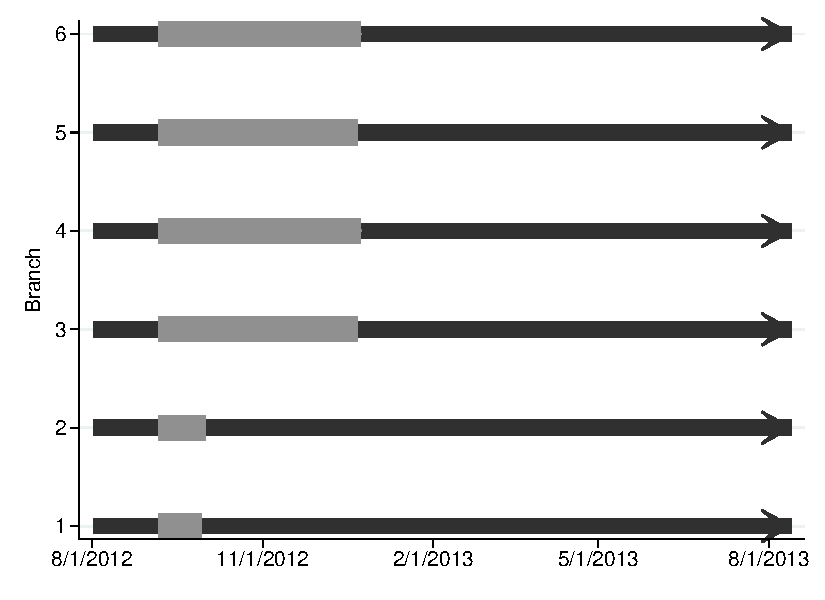
\includegraphics[width=\textwidth]{Figuras/timeline_suc_exp_extended.pdf}
    \end{subfigure}
    \begin{subfigure}{0.45\textwidth}
    \caption{Experiment arms}
       \centering
      \includegraphics[width=\textwidth]{Figuras/exp_arms.PNG}
    \end{subfigure}
    \end{center}
         \scriptsize Panel (a) displays in black arrows the period covered by our administrative data: from \hl{XXX} (\hl{XXX} days before the experiment began) to \hl{XXX}. The gray lines arrows correspond to the dates of implementation of the experiment. We finished the experiment earlier in branches 1 and 2 because we realized that we would have enough sample size with the remaining branches and save on operational costs. Panel (b) shows our 5 treatment arms: control (status quo contract), no choice with fee, no choice with promise, choice among both contracts where the commitment contract has fee, and choice among both contracts where the commitment contract involves only a promise. Within each arm it displays the number of observations. And  for the Choice groups it splits the sample size into those who chose the commitment contract (shaded blue triangle) and those that did not (un-shaded triangle).
      \textit{Do file: }  \texttt{timeline\_suc\_exp.do}
\end{figure}




\begin{figure}[H]
     \caption{Financial cost}
    \label{fc_hist}
    \begin{center}
    \begin{subfigure}{.45\textwidth}
      \caption{In pesos}
        \centering
        \includegraphics[width=\textwidth]{Figuras/hist_fc.pdf}
    \end{subfigure}
    \begin{subfigure}{0.45\textwidth}
    \caption{As a fraction of the loan}
       \centering
      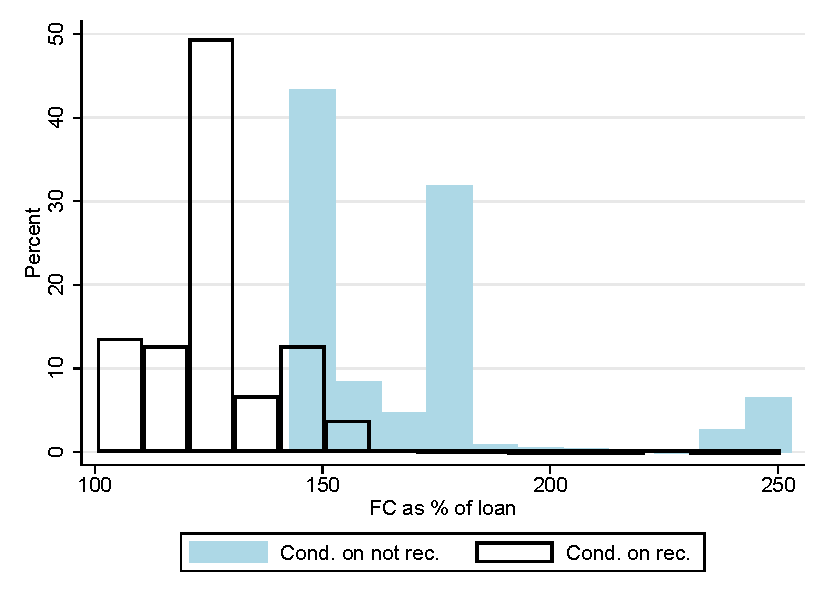
\includegraphics[width=\textwidth]{Figuras/hist_fc_perc_loan.pdf}
    \end{subfigure}
    \end{center}
         \scriptsize
         Panel (a) presents a histogram of financial cost for \hl{the control group}. Financial cost is defined as the sum of payments made by a client towards recovering her pawn + the cost of the pawn in case she ends up losing it. In the paper we use different costs of losing the pawn: its value in gold, and the subjective value given (jewelry may have sentimental value). This figure uses the \hl{gold value}. We plot separately the financial cost for those who lose the pawn (blue) and those that recover it (transparent).  Panel (b) is analogous but normalized the financial cost dividing by the loan size.  Given that the loan lasts close to 90 days, bringing payments to present value makes little difference. 
      \footnotesize{ } \textit{Do file: }  \texttt{hist\_fc.do}
\end{figure}




\begin{figure}[H]
    \caption{Behavior of those who lost pawn}
    \label{proxy_naive}
    \begin{center}
    \begin{subfigure}{0.40\textwidth}
        \caption{Elapsed days to first payment}
        \centering
        \includegraphics[width=\textwidth]{Figuras/hist_firstdays_default.pdf}
    \end{subfigure}
    \begin{subfigure}{0.40\textwidth}
        \caption{Elapsed days to last payment}
        \centering
        \includegraphics[width=\textwidth]{Figuras/hist_days_default.pdf}
    \end{subfigure}
        \begin{subfigure}{0.40\textwidth}
        \caption{Payments as \% of loan}
        \centering
        \includegraphics[width=\textwidth]{Figuras/hist_percpay_default.pdf}
    \end{subfigure}
    \begin{subfigure}{0.40\textwidth}
        \caption{Number of payments}
        \centering
        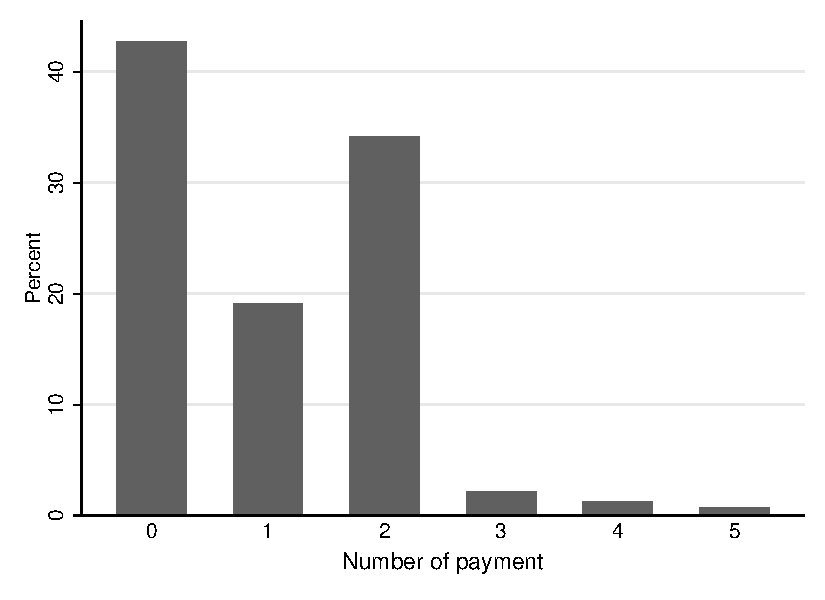
\includegraphics[width=\textwidth]{Figuras/hist_numpay_default.pdf}
    \end{subfigure}
    \end{center}
        \scriptsize 
        This figure describes behavior for the subsample of clients whose pawn was not recovered.  Panel (a) shows days elapsed from the pawn to the first payment, while panel (b) displays the days elapsed to last payment. Some people pay after the day 105 when the grace period ends because the can ``restart'' the loan if they pay all interest owed. It amount to starting a new loan \hl{with the same conditions} and same pawn. Panel (c) shows the the fraction of the loan that they paid already, even when they ended up losing the pawn. Panel (d) displays the number of times they went to the branch to pay.      
      \textit{Do file: }  \texttt{hist\_den\_default.do}
\end{figure}




\begin{figure}[H]
    \caption{The effect of ``forcing'' (with fees)}
    \label{fc_pro2}
    \begin{center}
    \begin{subfigure}{0.45\textwidth}
        \caption{Financial cost}
        \centering
        \includegraphics[width=\textwidth]{Figuras/fc_te_pro_2.pdf}
    \end{subfigure}
        \begin{subfigure}{0.45\textwidth}
        \caption{Financial Cost (quantile reg)}
        \centering
        \includegraphics[width=\textwidth]{Figuras/fc_quantile_pro_2.pdf}
    \end{subfigure}
    \begin{subfigure}{0.55\textwidth}
        \caption{Lost Pawn}
        \centering
        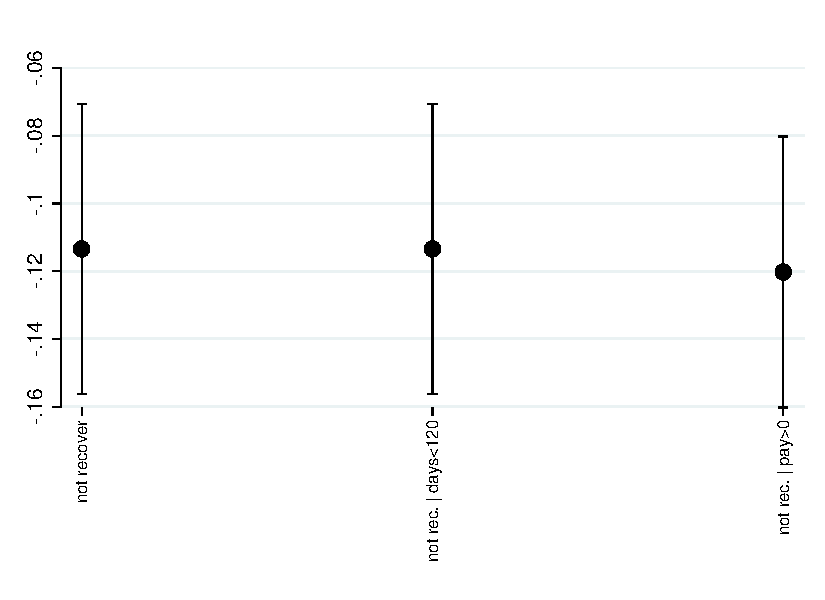
\includegraphics[width=\textwidth]{Figuras/def_te_pro_2.pdf}
    \end{subfigure}
    \end{center}
        \scriptsize
        This figure shows the estimated treatment effect of ``forcing'' the frequent payment commitment contract compared to the status-quo (control) for our two main outcomes: financial cost (Panel a), quantiles of financial cost (Panel b), and for and an indicator for losing the pawn (Panel c). Each dot represents the estimated treatment effect of a different regression (or sub-population) and its 95\% confidence interval. In Panel (a), the first effect corresponds to using the gold value of the pawn in the definition of financial cost and discounting the payments to present value; the second uses the subjective value of the pawn in the definition of financial cost; the third is analogous to the second but adds transaction cost (transport+1 day wage) per visit to the cost, to it involves both financial cost and transport + opportunity cost; the fourth conditions on the population that paid any positive amount towards recovery of their pawn; the fifth conditions on the sub-population \hl{of the treatment group} that paid a fee and \hl{compares these to all the control group}; the sixth conditions on the intersection of the previous two sub-populations; the seventh conditions on those we classify as overconfident (by comparing their subjective prediction of recovering their pawn versus a machine learning prediction using observables, both from the baseline survey); the seventh is focuses on non-overconfident; and the last one conditions on those we classify as present biased using the baseline survey. Panel (b) plots the effects on   on different quantiles of the distribution of financial cost (\hl{defined using the first definition}): 15th, 25th, 50th, 75th, 85th percentile. Panel (c) has to parts and to y-axis scales. The left Y-axis measures the effect of treatment on losing their pawn and has 8 coefficients. The first coefficient compares all the treatment group vs all the control; the second conditions on the population that paid any positive amount towards recovery of their pawn; the third conditions on having paid at least 30\% of the loan amount; the fourth conditions on the period covering the first cycle of the loan; the fifth on the period of the first cycle and paying any positive amount; the sixth, seventh and eight on overconfident, non-overconfident, and present biased as defined above in this note. The right Y-axis of Panel (c) measures the likelihood doing an additional pawn in the period of 75 days and after the pawn in the treatment and control groups. That is it measures the effect on ``repeat purchase'' of having been subjected to treatment for at least 75 days.
      \textit{Do file: }  \texttt{fc\_te.do, def\_te.do, fc\_quantilereg.do}
\end{figure}



\begin{figure}[H]
    \caption{Relationship between treatment effects}
    \label{binscatter}
    \begin{center}
    \begin{subfigure}{0.45\textwidth}
        \caption{\footnotesize{Induced to pay earlier and Induced Lower FC}}
        \centering
        \includegraphics[width=\textwidth]{Figuras/binscatter_fc_days_pro_2.pdf}
    \end{subfigure}
        \begin{subfigure}{0.45\textwidth}
        \caption{\footnotesize{Induced to pay earlier and Induced Recovery}}
        \centering
        \includegraphics[width=\textwidth]{Figuras/binscatter_def_days_pro_2.pdf}
    \end{subfigure}
    \end{center}
       \scriptsize 
       This figure plots relationships between \textit{treatment effects}. Both Panels (a) an (b) have the same X-axis, which displays the estimated heterogeneous treatment effect on the outcome ``elapsed days of first payment'', that is how many days elapsed from the day the loan was awarded to the first payment the client made. The treatments effects were calculated using Athey and Wagner (\hl{YEAR XXX}). We use command \hl{XXX} in $R$ which outputs an estimated treatment effect for each person in treatment and control. In Panel (a) the Y-Axis is the \textit{treatment effect} on financial cost. In Panel (b) the Y-axis is the \textit{treatment effect} on losing their pawn. Panel (a) shows that those induced to pay earlier are also those that have larger savings in financial cost as a result of ``forcing'' the frequent payment commitment contract compared to the status-quo (control). Panel (b) shows that those induced to pay earlier are also those that have a larger increase in recovery.
      \textit{Do file: }  \texttt{binscatter\_hte.do}
\end{figure}






\begin{figure}[H]
    \caption{The Effect of choice (with fees)}
    \label{fc_pro4}
    \begin{center}
    \begin{subfigure}{0.45\textwidth}
        \caption{Financial cost}
        \centering
        \includegraphics[width=\textwidth]{Figuras/fc_te_pro_4.pdf}
    \end{subfigure}
        \begin{subfigure}{0.45\textwidth}
        \caption{Financial Cost (quantile reg)}
        \centering
        \includegraphics[width=\textwidth]{Figuras/fc_quantile_pro_4.pdf}
    \end{subfigure}
    \begin{subfigure}{0.60\textwidth}
        \caption{Lost Pawn}
        \centering
        \includegraphics[width=\textwidth]{Figuras/def_te_pro_4.pdf}
    \end{subfigure}
    \end{center}
        \scriptsize
        This figure is analogous to Figure \ref{fc_pro2}. It measures the effect of being given \textit{choice} between the frequent payment commitment contract and the status-quo contract versus being \textit{``forced''} into the status-quo contract (control). Again it focuses our two main outcomes: financial cost and an indicator for losing the pawn. However, it also presents differences in these two outcomes for those who chose the frequent payment commitment contract versus the whole control group (squares-NSQ), and also for those who chose the status quo contract versus the whole control group (triangles-SQ). Note that these two comparisons are not pure causal effects since people who chose the frequent payment commitment contract may be different from those that do not. That is: the squares and triangles combine selection and treatment effects. Finally, for comparison purposes, the blue diamonds display the effects of forcing them into the frequent payment commitment contract and are just transcribed from Figure \ref{fc_pro2} above. 
      \textit{Do file: }  \texttt{fc\_te\_choice\_dec.do, def\_te\_choice\_dec.do, fc\_quantilereg\_choice\_dec.do}
\end{figure}



\begin{figure}[H]
    \caption{Who makes mistakes?}
    \label{choose_wrong}
    \begin{center}
    \begin{subfigure}{0.4\textwidth}
        \caption{\footnotesize{Effect of losing pawn vs predicted take-up}}
        \centering
        \includegraphics[width=\textwidth]{Figuras/takeuppr_def.pdf}
    \end{subfigure}
        \begin{subfigure}{0.5\textwidth}
        \caption{\footnotesize{Chose wrong}}
        \centering
        \includegraphics[width=\textwidth]{Figuras/line_cw_pw_fc_te_cf.pdf}
    \end{subfigure}
    \end{center}
             \scriptsize
             Panel (a) estimates the treatment effect of forcing the frequent payment commitment contract on the probability of losing the pawn. It does this for sub-populations defined in terms of the predicted probability of taking up the frequent payment commitment contract \textit{had they been given the choice}. We calculate the probability using observed take up in the choice arm by the method of random forests using baseline survey and admin data. Then we extrapolate these predictions to the no-choice arm and group clients (in treatment and control) into 5 groups according to whether their predicted probability $\hat{P(x_i)}$ is in \hl{[0,10],(10,20],(50,70],(30,}. For each of these groups separately we estimate the ATE using regression equation \hl{XXX}.  The non-monotonicity indicates that take up of treatment is \textit{not} strongly correlated with the benefit of treatment. \hl{Panel (b) works within the choice-group;} for them we observe take up of treatment. We then impute counterfactual treatment effects \hl{estimated in the no-choice group} and extrapolated to the choice-group using the observables. So we have an estimate of what would have happened if client $i$ had chosen otherwise. More concretely, for each client we calculate two numbers: what fraction would have done better with the contract the did not chose (Y-axis on the left), and how much financial cost would they save with this other contract (Y-axis on the right). The X-axis displays the treshold of what we classify as a ``mistake'' The red lines do this for the choice group with fee-commitment and the blue lines do this with the choice group with promise-commitment. We estimate that about 10\% made mistakes betwee
             
             \textit{Do file: }  \texttt{effect\_contr\_takeup.do, choose\_wrong\_quant\_wrong.do}
\end{figure}







\begin{figure}[H]
    \caption{“Forced commitment with promise Treatment Effects}
    \label{fc_pro3}
    \begin{center}
    \begin{subfigure}{0.45\textwidth}
        \caption{Financial cost}
        \centering
        \includegraphics[width=\textwidth]{Figuras/fc_te_pro_3.pdf}
    \end{subfigure}
        \begin{subfigure}{0.45\textwidth}
        \caption{Quantile regression}
        \centering
        \includegraphics[width=\textwidth]{Figuras/fc_quantile_pro_3.pdf}
    \end{subfigure}
    \begin{subfigure}{0.55\textwidth}
        \caption{Not recovery}
        \centering
        \includegraphics[width=\textwidth]{Figuras/def_te_pro_3.pdf}
    \end{subfigure}
    \end{center}
             \footnotesize \textit{Notes: } 
      \footnotesize{ } \textit{Do file: }  \texttt{fc\_te.do, def\_te.do, fc\_quantilereg.do}
\end{figure}





\begin{figure}[H]
    \caption{Voluntary commitment with promise” Treatment Effects}
    \label{fc_pro5}
    \begin{center}
    \begin{subfigure}{0.45\textwidth}
        \caption{Financial cost}
        \centering
        \includegraphics[width=\textwidth]{Figuras/fc_te_pro_5.pdf}
    \end{subfigure}
        \begin{subfigure}{0.45\textwidth}
        \caption{Quantile regression}
        \centering
        \includegraphics[width=\textwidth]{Figuras/fc_quantile_pro_5.pdf}
    \end{subfigure}
    \begin{subfigure}{0.45\textwidth}
        \caption{Not recovery}
        \centering
        \includegraphics[width=\textwidth]{Figuras/def_te_pro_5.pdf}
    \end{subfigure}
    \end{center}
             \footnotesize \textit{Notes: } 
      \footnotesize{ } \textit{Do file: }  \texttt{fc\_te\_choice\_dec.do, def\_te\_choice\_dec.do, fc\_quantilereg\_choice\_dec.do}
\end{figure}


\pagebreak


%%%%%%%%%%%%%%%%%%%%%%%%%%%%%%%%%%%%%%%%%%%%%%%

% APPENDIX TABLES

\section{APPENDIX}

\subsection{Tables}


\begin{table}[H]
    \caption{Out of sample measures of fit}
    \label{Table_compliance}
    \begin{subtable}{1\textwidth}
      \centering
        \caption{Take up}
        \scriptsize{% Table generated by Excel2LaTeX from sheet 'oos_pago_frec_vol'
\begin{tabular}{lcccc}
\toprule
      & \multicolumn{4}{c}{Choice} \\
\midrule
\midrule
GOF measures & Logit & SW-Logit & RF    & Boosting \\
\midrule
\midrule
AUC (out of sample) & 0.77  & 0.76  & 0.8   & 0.77 \\
      & (0.04) & (0.04) & (0.04) & (0.04) \\
AUC (in sample) & 0.76  & 0.75  & 0.87  & 0.84 \\
      & (0.02) & (0.02) & (0.01) & (0.01) \\
Accuracy & 0.77  & 0.78  & 0.75  & 0.78 \\
\bottomrule
\bottomrule
\end{tabular}%
}
    \end{subtable}%
    
    \bigskip
    \begin{subtable}{1\textwidth}
      \centering
        \caption{Take up w/Fee}
        \scriptsize{% Table generated by Excel2LaTeX from sheet 'oos_pago_frec_vol_fee'
\begin{tabular}{lcccc}
\toprule
      & \multicolumn{4}{c}{Frequent voluntary payment - FEE} \\
\midrule
\midrule
OOS measures & Logit & SW-Logit & RF    & Boosting \\
\midrule
\midrule
MAE   & 0.21  & 0.21  & 0.23  & 0.17 \\
MSE   & 0.1   & 0.1   & 0.1   & 0.09 \\
AUC (out of sample) & 0.76  & 0.78  & 0.84  & 0.85 \\
      & (0.06) & (0.06) & (0.06) & (0.05) \\
AUC (in sample) & 0.84  & 0.82  & 0.92  & 0.99 \\
      & (0.02) & (0.02) & (0.01) & (0.01) \\
Accuracy & 0.82  & 0.84  & 0.86  & 0.88 \\
Correlation (0-1) & 0.13  & 0.26  & 0.37  & 0.31 \\
Correlation (predicted val) & 0.33  & 0.38  & 0.37  & 0.43 \\
R-squared  & 0.08  & 0.13  & 0.11  & 0.19 \\
Expected value of predictions & 0.17  & 0.17  & 0.16  & 0.12 \\
\bottomrule
\bottomrule
\end{tabular}%
}
    \end{subtable}
    
      \bigskip
    \begin{subtable}{1\textwidth}
      \centering
        \caption{Take up w/promise}
        \scriptsize{% Table generated by Excel2LaTeX from sheet 'oos_pago_frec_vol_promise'
\begin{tabular}{lcccc}
\toprule
      & \multicolumn{4}{c}{Choice-Promise Arm} \\
\midrule
\midrule
GOF measures & Logit & SW-Logit & RF    & Boosting \\
\midrule
\midrule
AUC (out of sample) & 0.63  & 0.63  & 0.7   & 0.72 \\
      & (0.06) & (0.06) & (0.06) & (0.06) \\
AUC (in sample) & 0.83  & 0.82  & 0.9   & 0.97 \\
      & (0.02) & (0.02) & (0.01) & (0.01) \\
Accuracy & 0.62  & 0.67  & 0.65  & 0.7 \\
\bottomrule
\bottomrule
\end{tabular}%
}
    \end{subtable}
            \scriptsize
           \\
           \\
           \\
  \textit{Notes:} 
    
     \textit{Scripts: } \texttt{pred\_take\_up.do, pfv\_pred.R}
\end{table}



\begin{table}[H]
\caption{Summary statistics (exit survey)}
\label{SS_exit}
\begin{center}
\scriptsize{% Table generated by Excel2LaTeX from sheet 'SS'
\begin{tabular}{lccccccc}
\toprule
\multicolumn{8}{c}{Exit Survey Data} \\
\midrule
\midrule
      &       &       & \multicolumn{2}{c}{No Choice } & \multicolumn{2}{c}{Choice} &  \\
\midrule
\midrule
      & Overall & Control & Fee   & Promise & Fee   & Promise & p-value \\
\midrule
      & \multicolumn{7}{c}{Panel A: Outcomes} \\
\midrule
\midrule
Will reincide & 0.94  & 0.96  & 0.95  & 0.96  & 0.94  & 0.92  & 0.6 \\
      & (0.01) & (0.01) & (0.02) & (0.02) & (0.02) & (0.03) &  \\
Very satisfied & 0.34  & 0.36  & 0.32  & 0.33  & 0.33  & 0.36  & 0.95 \\
      & (0.02) & (0.05) & (0.05) & (0.05) & (0.04) & (0.04) &  \\
Better econ situation & 0.42  & 0.53  & 0.29*** & 0.35** & 0.44  & 0.47  & 0.02 \\
      & (0.03) & (0.06) & (0.05) & (0.06) & (0.05) & (0.04) &  \\
Choose frequent payment & 0.63  & 0.65  & 0.58  & 0.58  & 0.58  & 0.77** & 0 \\
      & (0.02) & (0.05) & (0.05) & (0.06) & (0.04) & (0.03) &  \\
\midrule
      & \multicolumn{7}{c}{Panel B: Balance} \\
\midrule
\midrule
Loan amount  & 1957.72 & 1940.41 & 1926  & 2006.83 & 2002.97 & 1892.54 & 0.98 \\
      & (67.84) & (160.03) & (150.89) & (187.56) & (114.96) & (157.83) &  \\
Woman & 0.71  & 0.69  & 0.72  & 0.77  & 0.66  & 0.73  & 0.58 \\
      & (0.02) & (0.05) & (0.06) & (0.05) & (0.05) & (0.04) &  \\
Age   & 43.98 & 42.84 & 46.27 & 43.82 & 44.57 & 42.24 & 0.29 \\
      & (0.59) & (1.33) & (1.74) & (1.1) & (0.99) & (1.16) &  \\
Subjective value & 3166.31 & 3448.99 & 3182.11 & 3049.88 & 3074.69 & 3081.52 & 0.85 \\
      & (120.82) & (288.38) & (286.2) & (303.87) & (210.79) & (296.63) &  \\
Has pawn before & 0.88  & 0.84  & 0.9   & 0.87  & 0.95** & 0.8   & 0.01 \\
      & (0.02) & (0.05) & (0.03) & (0.05) & (0.02) & (0.05) &  \\
Subj. pr. of recovery & 95.35 & 94.5  & 94.84 & 96.6  & 95.06 & 95.87 & 0.82 \\
      & (0.56) & (1.4) & (1.21) & (1.5) & (1.01) & (1.09) &  \\
+High-school & 0.66  & 0.72  & 0.63  & 0.65  & 0.67  & 0.64  & 0.84 \\
      & (0.03) & (0.06) & (0.06) & (0.07) & (0.05) & (0.06) &  \\
\midrule
Obs   & 905   & 175   & 154   & 172   & 234   & 170   &  \\
\bottomrule
\bottomrule
\end{tabular}%
}
\end{center}
 \footnotesize
\textit{Notes:} 

\textit{Do file: } \texttt{ss.do}
\end{table}


\pagebreak



\subsection{Figures}



\begin{figure}[H]
     \caption{Booklet: Choice days}
    \label{booklet_translate}
    \begin{center}
    %\begin{subfigure}{0.55\textwidth}
    %    \centering
    %    \includegraphics[width=\textwidth]{Figuras/MP_F.pdf}
    %\end{subfigure}
    \begin{subfigure}{0.8\textwidth}
        \centering
        \includegraphics[width=\textwidth]{Figuras/MP_2.pdf}
    \end{subfigure}
    \end{center}
\end{figure}



\begin{figure}[H]
        \caption{Histogram of payments}
    \label{HistPayments}
    \begin{center}
        \centering
        \includegraphics[width=\textwidth]{hist_payments.pdf}
    \end{center}
     \footnotesize \textit{Notes: } 
      \footnotesize{ \textit{Do file: }  \texttt{hist\_payments.do}}
\end{figure}

\begin{figure}[H]
        \caption{Types of agents that incur in different FC}
    \label{components_fc}
    \begin{center}
        \centering
        \includegraphics[width=\textwidth]{Figuras/scatter_fc_pay.pdf}
    \end{center}
     \footnotesize \textit{Notes: } 
      \footnotesize{ \textit{Do file: }  \texttt{hist\_fc.do}}
\end{figure}

\begin{figure}[H]
        \caption{Percentage of payments}
    \label{Percentage_payments}
    \begin{center}
        \centering
        \includegraphics[width=\textwidth]{Figuras/hist_perc_payment.pdf}
    \end{center}
     \footnotesize \textit{Notes: } 
      \footnotesize{ \textit{Do file: }  \texttt{hist\_perc\_payment.do}}
\end{figure}


\begin{figure}[H]
    \caption{Evolution of payment}
    \label{Evolution payment}
    \begin{center}
    \begin{subfigure}{0.49\textwidth}
        \caption{Paid loans}
        \centering
        \includegraphics[width=\textwidth]{Figuras/desempeno_evol.pdf}
    \end{subfigure}
     \begin{subfigure}{0.49\textwidth}
      \caption*{}
        \centering
        \includegraphics[width=\textwidth]{Figuras/desempeno_evol_choice.pdf}
    \end{subfigure}
    
     \begin{subfigure}{0.49\textwidth}
        \caption{Average percentage of paid loans}
        \centering
        \includegraphics[width=\textwidth]{Figuras/sum_porc_evol.pdf}
    \end{subfigure}
     \begin{subfigure}{0.49\textwidth}
      \caption*{}
        \centering
        \includegraphics[width=\textwidth]{Figuras/sum_porc_evol_choice.pdf}
    \end{subfigure}
    
    \begin{subfigure}{0.49\textwidth}
        \caption{Average percentage of paid loans (condition on paid loan)}
        \centering
        \includegraphics[width=\textwidth]{Figuras/sum_porc_cond_evol.pdf}
    \end{subfigure}
     \begin{subfigure}{0.49\textwidth}
      \caption*{}
        \centering
        \includegraphics[width=\textwidth]{Figuras/sum_porc_cond_evol_choice.pdf}
    \end{subfigure}
    \end{center}
     \footnotesize \textit{Notes: } 
      \footnotesize{ \textit{Do file: }  \texttt{evol\_payment.do}}
\end{figure}



\begin{figure}[H]
    \caption{Heterogeneous Treatment Effect - NoChoice/Fee}
    \label{heterogeneous_te_3}
    \begin{center}
    \begin{subfigure}{0.4\textwidth}
        \caption{Financial cost}
        \centering
        \includegraphics[width=\textwidth]{Figuras/he_dist_fc_admin_disc_pro_2.pdf}
    \end{subfigure}
    \begin{subfigure}{0.4\textwidth}
        \caption*{}
        \centering
        \includegraphics[width=\textwidth]{Figuras/HE/he_int_vertical_fc_admin_disc_pro_2.pdf}
    \end{subfigure}
    
    \begin{subfigure}{0.4\textwidth}
        \caption{Not recovery}
        \centering
        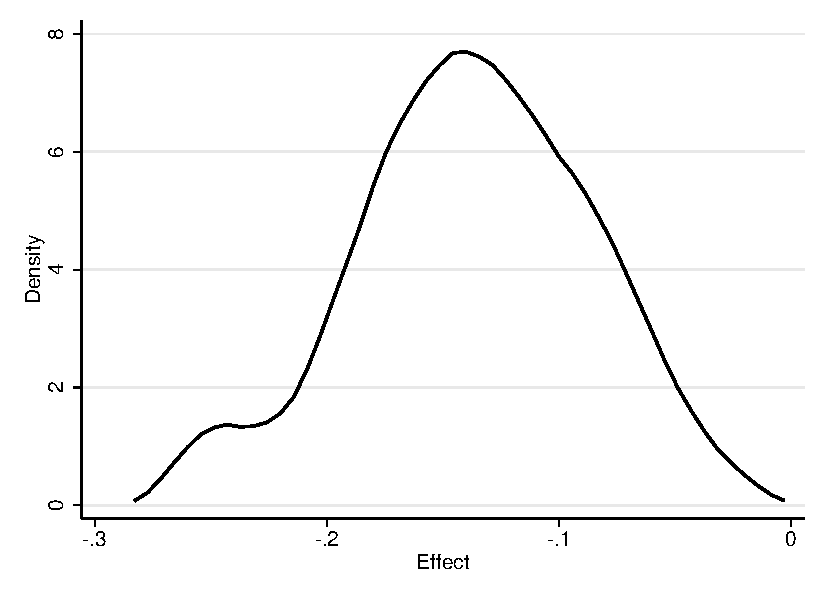
\includegraphics[width=\textwidth]{Figuras/he_dist_def_c_pro_2.pdf}
    \end{subfigure}
    \begin{subfigure}{0.4\textwidth}
        \caption*{}
        \centering
        \includegraphics[width=\textwidth]{Figuras/HE/he_int_vertical_def_c_pro_2.pdf}
    \end{subfigure}
    \end{center}
     \footnotesize \textit{Notes: } 
      \footnotesize{ \textit{Do file: }  \texttt{analyze\_grf\_single\_arm.do}}
\end{figure}


\begin{figure}[H]
        \caption{Heterogeneous treatment effect (NoChoice/Fee) decomposed by recovery}
    \label{hte_dec_rec}
    \begin{center}
        \centering
        \includegraphics[width=\textwidth]{Figuras/he_dist_dec_fc_admin_disc_pro_2.pdf}
    \end{center}
     \footnotesize \textit{Notes: } 
        \footnotesize{ } \textit{Do file: }  \texttt{analyze\_grf\_single\_arm.do.do}
\end{figure}






\begin{figure}[H]
    \caption{Heterogeneous Treatment Effect - NoChoice/Promise}
    \label{heterogeneous_te_3}
    \begin{center}
    \begin{subfigure}{0.4\textwidth}
        \caption{Financial cost}
        \centering
        \includegraphics[width=\textwidth]{Figuras/he_dist_fc_admin_disc_pro_3.pdf}
    \end{subfigure}
    \begin{subfigure}{0.4\textwidth}
        \caption*{}
        \centering
        \includegraphics[width=\textwidth]{Figuras/HE/he_int_vertical_fc_admin_disc_pro_3.pdf}
    \end{subfigure}
    
    \begin{subfigure}{0.4\textwidth}
        \caption{Not recovery}
        \centering
        \includegraphics[width=\textwidth]{Figuras/he_dist_def_c_pro_3.pdf}
    \end{subfigure}
    \begin{subfigure}{0.4\textwidth}
        \caption*{}
        \centering
        \includegraphics[width=\textwidth]{Figuras/HE/he_int_vertical_def_c_pro_3.pdf}
    \end{subfigure}
    \end{center}
     \footnotesize \textit{Notes: } 
      \footnotesize{ \textit{Do file: }  \texttt{analyze\_grf\_single\_arm.do}}
\end{figure}




\begin{figure}[H]
    \caption{Heterogeneous Treatment Effect - Choice/Fee}
    \label{heterogeneous_te_4}
    \begin{center}
    \begin{subfigure}{0.4\textwidth}
        \caption{Financial cost}
        \centering
        \includegraphics[width=\textwidth]{Figuras/he_dist_fc_admin_disc_pro_4.pdf}
    \end{subfigure}
    \begin{subfigure}{0.4\textwidth}
        \caption*{}
        \centering
        \includegraphics[width=\textwidth]{Figuras/HE/he_int_vertical_fc_admin_disc_pro_4.pdf}
    \end{subfigure}
    
    \begin{subfigure}{0.4\textwidth}
        \caption{Not recovery}
        \centering
        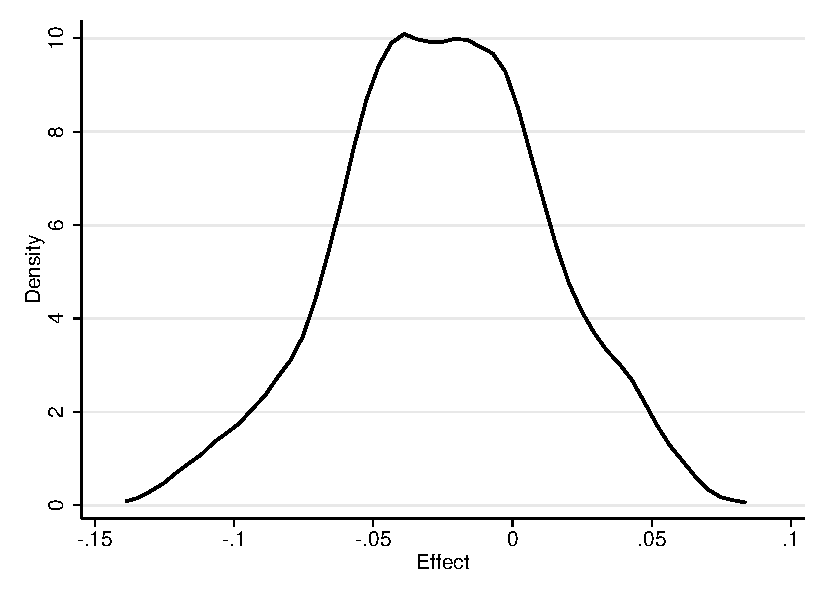
\includegraphics[width=\textwidth]{Figuras/he_dist_def_c_pro_4.pdf}
    \end{subfigure}
    \begin{subfigure}{0.4\textwidth}
        \caption*{}
        \centering
        \includegraphics[width=\textwidth]{Figuras/HE/he_int_vertical_def_c_pro_4.pdf}
    \end{subfigure}
    \end{center}
     \footnotesize \textit{Notes: } 
      \footnotesize{ \textit{Do file: }  \texttt{analyze\_grf\_single\_arm.do}}
\end{figure}



\begin{figure}[H]
    \caption{Heterogeneous Treatment Effect - Choice/Promise}
    \label{heterogeneous_te_5}
    \begin{center}
    \begin{subfigure}{0.4\textwidth}
        \caption{Financial cost}
        \centering
        \includegraphics[width=\textwidth]{Figuras/he_dist_fc_admin_disc_pro_5.pdf}
    \end{subfigure}
    \begin{subfigure}{0.4\textwidth}
        \caption*{}
        \centering
        \includegraphics[width=\textwidth]{Figuras/HE/he_int_vertical_fc_admin_disc_pro_5.pdf}
    \end{subfigure}
    
    \begin{subfigure}{0.4\textwidth}
        \caption{Not recovery}
        \centering
        \includegraphics[width=\textwidth]{Figuras/he_dist_def_c_pro_5.pdf}
    \end{subfigure}
    \begin{subfigure}{0.4\textwidth}
        \caption*{}
        \centering
        \includegraphics[width=\textwidth]{Figuras/HE/he_int_vertical_def_c_pro_5.pdf}
    \end{subfigure}
    \end{center}
     \footnotesize \textit{Notes: } 
      \footnotesize{ \textit{Do file: }  \texttt{analyze\_grf\_single\_arm.do}}
\end{figure}


\begin{figure}[H]
    \caption{Take-up Fee against HTE}
    \label{takeup_hte}
    \begin{center}
    \begin{subfigure}{0.45\textwidth}
        \caption{Paid loan - Fee}
        \centering
        \includegraphics[width=\textwidth]{Figuras/takeup_he_pro_2_pago_frec_vol_fee_des_c.pdf}
    \end{subfigure}
    \begin{subfigure}{0.45\textwidth}
        \caption{Paid loan - Promise}
        \centering
        \includegraphics[width=\textwidth]{Figuras/takeup_he_pro_3_pago_frec_vol_fee_des_c.pdf}
    \end{subfigure}
    
        \begin{subfigure}{0.45\textwidth}
        \caption{FC subjective - Fee}
        \centering
        \includegraphics[width=\textwidth]{Figuras/takeup_he_pro_2_pago_frec_vol_fee_fc_survey.pdf}
    \end{subfigure}
    \begin{subfigure}{0.45\textwidth}
        \caption{FC subjective - Promise}
        \centering
        \includegraphics[width=\textwidth]{Figuras/takeup_he_pro_3_pago_frec_vol_fee_fc_survey.pdf}
    \end{subfigure}
   
        \begin{subfigure}{0.45\textwidth}
        \caption{Total Payment - Fee}
        \centering
        \includegraphics[width=\textwidth]{Figuras/takeup_he_pro_2_pago_frec_vol_fee_sum_p_c.pdf}
    \end{subfigure}
    \begin{subfigure}{0.45\textwidth}
        \caption{Total Payment - Promise}
        \centering
        \includegraphics[width=\textwidth]{Figuras/takeup_he_pro_3_pago_frec_vol_fee_sum_p_c.pdf}
    \end{subfigure}    
    
    
    \end{center}
     \footnotesize \textit{Notes: } 
      \footnotesize{ \textit{Do file \& RScripts: }  \texttt{heffect\_takeup\_nochoicearm.do, pfv\_pred\_hte.R}}
\end{figure}






\begin{figure}[H]
    \caption{Reasons to pawn or not again with monthly payments}
    \label{reasons}
    \begin{center}
    \begin{subfigure}{0.5\textwidth}
        \caption{Pawn again because:}
        \centering
        \includegraphics[width=\textwidth]{Figuras/razones_si.pdf}
    \end{subfigure}
    \begin{subfigure}{0.5\textwidth}
        \caption{Not pawn because:}
        \centering
        \includegraphics[width=\textwidth]{Figuras/razones_no.pdf}
    \end{subfigure}
    \end{center}
     \footnotesize \textit{Notes: } 
      \footnotesize{ \textit{Do file: }  \texttt{ss.do}}
\end{figure}

\begin{figure}[H]
    \caption{Voluntary take up of monthly payment}
    \label{interactions_takeup}
    \begin{center}
    \begin{subfigure}{0.8\textwidth}
        \caption{``with Fee'' Arm}
        \centering
        \includegraphics[width=\textwidth]{Figuras/pago_frec_vol_fee_interactions_rf.pdf}
    \end{subfigure}
    \begin{subfigure}{0.8\textwidth}
        \caption{``with Promise Arm''}
        \centering
        \includegraphics[width=\textwidth]{Figuras/pago_frec_vol_promise_interactions_rf.pdf}
    \end{subfigure}
    \end{center}
     \footnotesize \textit{Notes: } 
      \footnotesize{ \textit{Do file: }  \texttt{plot\_take\_up.do}}
\end{figure}



\begin{figure}[H]
        \caption{\% of payments conditional on payment $>$ 0 and no item back}
    \label{HistPayments_pos}
    \begin{center}
        \centering
        \includegraphics[width=\textwidth]{Figuras/hist_perc_payment_conditional.pdf}
    \end{center}
     \footnotesize \textit{Notes: } 
      \footnotesize{ \textit{Do file: }  \texttt{hist\_payments.do}}
\end{figure}


\begin{figure}[H]
        \caption{Booklet with product information}
    \label{micas}
    \begin{center}
        \centering
        \includegraphics[width=\textwidth]{micas.pdf}
    \end{center}
     \footnotesize \textit{Notes: } 
      \footnotesize{ }
\end{figure}


\begin{figure}[H]
    \caption{Propensity to take up the commitment device}
    \label{prop_take_up_hte}
    \begin{center}
     \begin{subfigure}{0.45\textwidth}
        \caption{Fee}
        \centering
        \includegraphics[width=\textwidth]{Figuras/takeup_fee_he.pdf}
    \end{subfigure}
     \begin{subfigure}{0.45\textwidth}
        \caption{Promise}
        \centering
        \includegraphics[width=\textwidth]{Figuras/takeup_promise_he.pdf}
    \end{subfigure}
\end{center}
     \footnotesize \textit{Notes: } 
      \footnotesize{ \textit{Do file: }  \texttt{heffect\_takeup.do}}
\end{figure}


\begin{figure}[H]
     \caption{Booklet with product information translated}
    \label{booklet_translate2}
    \begin{center}
    \begin{subfigure}{.9\textwidth}
        \centering
        \includegraphics[width=\textwidth]{Figuras/MP_F.pdf}
    \end{subfigure}
    %\begin{subfigure}{0.55\textwidth}
    %   \centering
    %  \includegraphics[width=\textwidth]{Figuras/MP_2.pdf}
    %\end{subfigure}
    \end{center}
\end{figure}



\end{document}